% change according to folder and file names
\ifpdf
    \graphicspath{{4/figures/PNG/}{4/figures/PDF/}{3/figures/}}
\else
    \graphicspath{{4/figures/EPS/}{4/figures/}}
\fi

%: ----------------------- contents from here ------------------------
\chapter{EAs, MAEAs and Ill-Conditioned problems} % top level followed by section, subsection
\label{VarCorrChapter}
%\begin{flushright}
%Any intelligent fool can make things  
%\linebreak
%bigger, more complex, and more violent. 
%\linebreak
%It takes a touch of genius, and a lot of  
%\linebreak
%courage, to move in the opposite direction.
%\linebreak
%Albert Einstein
%\end{flushright}

This chapter investigates the loss of efficiency of EAs and MAEAs when they are dealing with ill-conditioned optimization problems \cite{Salomon,Roy_2002a,Ghisu_2010}. Proposes and validates an original method to regain a major part of the lost, due to ill-conditioned optimization problems, efficiency and additionally a second method dedicated in the improvement of the metamodel prediction quality.

The source of lost efficiency of EAs and MAEAs can be traced back to two main reasons; a) the curse of dimensionality and b) ill-conditioned optimization problems.  Unfortunately, in their majority, engineering optimization problems belong in both of the aforementioned categories. 

The curse of dimensionality states that the difficulty to solve an optimization problem increases with respect to the problems dimension, that is the number of free variables (N). IN EAs that translates into the loss of efficiency (evolution slowdown) resulting form the increased N. In MAEAs the curse of dimensionality spreads, apart from the evolution, also to the use of metamodels where both training time and prediction error increasing due to the increased dimension. The loss of efficiency due to the ``bad'' metamodel predictions is superimposed to the loss due to the ``bad'' evolution therefore the effect of the curse of dimensionality in MAEAs is twofold.  Regarding curse of dimensionality a method (KBD) that efficiently reduces the dimension exploiting the knowledge contained in archived designs has been presented and validated in chapter 3.             

Ill-conditioned problems, on the other hand, are the problems that suffer form; a) anisotropic objective function (f) and b) non-separable objective function. The definitions of anisotropic f and non-separable f follow in section \ref{IllCon} and \ref{Nonsep} respectively. Dealing with ill-conditioned problems states that the difficulty to solve an optimization problem increases superlinearly with respect to the problems dimension (N).  IN EAs that translates into a superlinear evolution slowdown with respect to N thus magnifying the negative effects of the curse of dimensionality. Furthermore the anisotropic nature of the objective function leads to the notion of more and less important design variables (or, in the case of non-separable f, directions in the design space). The latter can be used to reduce N, via truncation of the less important variables, either during the optimization procedure (which is not the case in this thesis and could be a proposal for future work) or during the metamodel training phase so as to increase its prediction quality.       

\section{Ill-Conditioned optimization problems}
The definitions of a) anisotropic objective function and b) non-separable objective function that characterize the objective function of an ill-conditioned problem are presented. Later an investigation regarding the effects of ill-conditioned optimization problems on EA efficiency is carried out.  

\subsection{Anisotropic objective function}
\label{IllCon}
The term anisotropic objective function refers to the condition were the contribution to the objective function value is largely anisotropic for the different design variables or ,more precisely, directions in search space.

Regarding the convex-quadratic function $f (x) = 2x^THx$, where $H$ is a symmetric positive definite $N \times N$ matrix, the condition number ($a$) of $H$ is defined as the ratio between its largest and smallest eigenvalue. The aforementioned eigenvalues correspond to the squared relative lengths of the principal axes of the ellipsoid $x^THx = 1$. For points located on the principal axes the gradient aligns with the axis direction, and the axis length determines the magnitude of movement required to achieve a certain change in f. Therefore f is said to be isotropic if the condition number of $H$ is equal to $a=1$ and anisotropic is $a>>>1$.

%In practise, an objective function is characterised as anisotropic, if for a given point the displacement that produces a certain function value improvement differs by orders of magnitude $a>10$.
  


\begin{figure}[h!]
\begin{minipage}[b]{1.0\linewidth}
 \centering
 \resizebox*{15cm}{!}{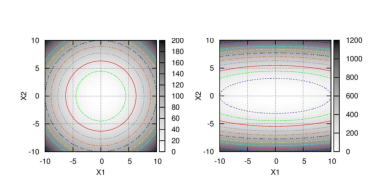
\includegraphics{ellipseA.eps}}
\end{minipage}
%\begin{minipage}[b]{0.5\linewidth}
% \centering
% \resizebox*{7.5cm}{!}{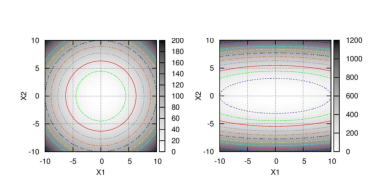
\includegraphics{ellipseA.eps}}
%\end{minipage}
\caption{Left: isotropic objective function with two design variables; the contribution of both $X_1$ and $X_2$ are the same. Right: anisotropic objective function; variable $X_2$ has higher contribution on the objective function than $X_1$.} 
\label{illc}
\end{figure}

In practise EAs are sophisticated enough to deal with anisotropic problems without loosing efficiency. Anisotropic objective functions, though, are prune to non-separability.         


\subsection{Non-separability}     
\label{Nonsep}
Separability of an objective function $f:\vec{x}\mapsto f(\vec{x})$ is a condition described for each and every variable $x_i \in \vec{x}$. An objective function is said to be separable with respect to $x_i$ if the optimal value of $x_i$ does not depend on the value  any other design variable takes on. A function $f$ is said to be separable if this is separable with respect to each and every member of $\vec{x}$.


\begin{figure}[h!]
\begin{minipage}[b]{1\linewidth}
 \centering
 \resizebox*{14cm}{!}{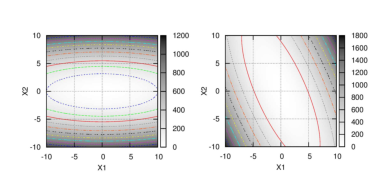
\includegraphics{ellipseB.eps}}
\end{minipage}
%\begin{minipage}[b]{0.5\linewidth}
% \centering
% \resizebox*{9cm}{!}{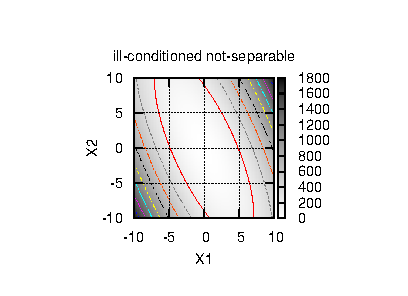
\includegraphics{ellipseturn.eps}}
%\end{minipage}
\caption{Left: Separable objective function. Right: Non-separable objective function.} 
\label{nonsep}
\end{figure}

Regarding non-separable objective functions, difficulty scales exponentially fast with the N since the search space volume increases exponentially with N. On the other hand, separable objective functions, even though the search space volume also increases exponentially with N, their difficulty scales only linearly with the search space dimension since the global optimum could be (theoretically) located by minimizing $n$ one dimensional objective functions (minimise $f_i(x_i),~ \forall x_i \in \vec{x}$).
 
\subsection{Investigation of ill-conditioned optimization problems on EA efficiency}
\label{Inv2}

In order to Investigate the effects of ill-conditioned optimization problems on EA efficiency two analytical test cases have been solved, for a range of design space dimensions, both in their separable and non-separable form. All the result that will be presented furthermore during this section are concerning the mean values over $10$ runs that took place with different random number generator seeds. 

The first analytical test case to me examined is a multidimensional ellipsoid (a 2d version of it can be seen in fig. \ref{nonsep}) described, in it separable form, by:   


\begin{eqnarray}
   f(\vec{x})=\sum^{n}_{i=1}=a^{\frac{i-1}{n-1}}x_i^2
   \label{ellipse} 
\end{eqnarray}
where $a$ is the so called condition number and controls the ill-conditioned state of the objective function. Large values of $a$ lead to increasingly ill-conditioned objective functions.

and in its non-separable form by:

\begin{eqnarray}
   f(\vec{x})=\sum^{n}_{i=1}=a^{\frac{i-1}{n-1}}y_i^2
   \label{ellipse} 
\end{eqnarray}
where $\vec{y}=B\vec{x}$ and $B$ a $n\times n$ orthogonal, rotation, matrix.

In order to investigate both the effects of the design space dimension ($n$) and the condition number ($a$) four different optimization problems will be solved. A ten dimensional ($n=10$) optimizations problem is solved for $a=10$ and $a=100$, see fig. \ref{ellipse_t1}, and a $n=30$ problem is solved for $a=100$ and $a=1000$, see fig. \ref{ellipse_t2}. 


\begin{figure}[h!]
\begin{minipage}[b]{0.5\linewidth}
 \centering
 \resizebox*{7.5cm}{!}{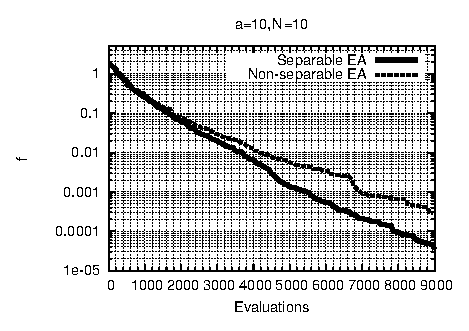
\includegraphics{10_10d.eps}}
\end{minipage}
\begin{minipage}[b]{0.5\linewidth}
 \centering
 \resizebox*{7.5cm}{!}{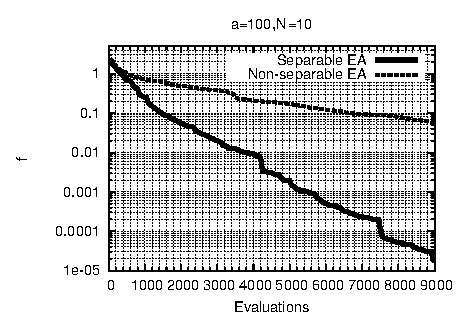
\includegraphics{100_10d.eps}}
\end{minipage}
\caption{Ten dimensional ellipsoid. Left: Condition number ($a=10$).  Right: Condition number ($a=100$). Increasing of $a$ for $10$ to $100$ causes additional losses and increases the performance gap between separable and non-separable optimization problem.} 
\label{ellipse_t1}
\end{figure}

\begin{figure}[h!]
\begin{minipage}[b]{0.5\linewidth}
 \centering
 \resizebox*{7.5cm}{!}{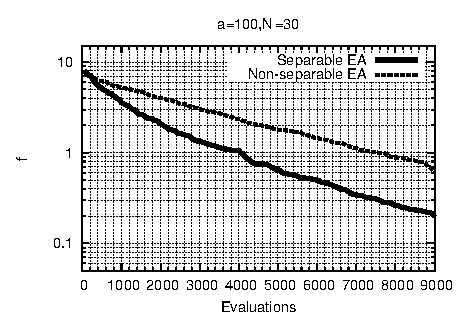
\includegraphics{100_30d.eps}}
\end{minipage}
\begin{minipage}[b]{0.5\linewidth}
 \centering
 \resizebox*{7.5cm}{!}{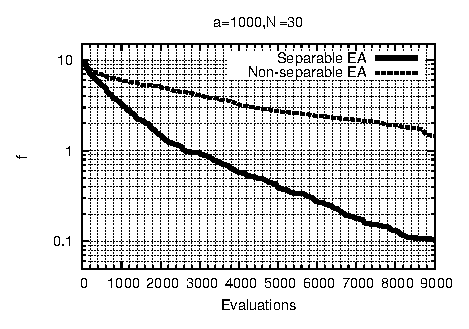
\includegraphics{1000_30d.eps}}
\end{minipage}
\caption{30 dimensional ellipsoid. Left: Condition number ($a=100$).  Right: Condition number ($a=1000$). Increasing of $a$ for $100$ to $1000$, as in the 10D case, causes additional losses and increases the performance gap between separable and non-separable optimization problem.} 

\label{ellipse_t2}
\end{figure}

Observing figures \ref{ellipse_t1} and \ref{ellipse_t2} one can identify both the effects of increased condition number and dimension. Bigger condition number leads to greater performance gab between separable and non-separable cases, for both the $n=10$ and $n=30$ cases. Bigger dimension also increases the gab between the two. Focusing on the $a=100$ case for both the $n=10$ and $n=30$ example once can observe that the difference of objective function values $\Delta(F)$, for the same computational cost of $9000$ evaluations, differ. For the $n=10$ case $\Delta(F)=F(non-separable)-F(separable) \approx  1e^{-4}$ on the other hand for the $n=30$ case $\Delta(F)=F(non-separable)-F(separable) \approx  0.9$. This difference of $\Delta(F)$ for the 10D and 30D case denotes a significant increase of the efficiency gab between separable and non-separable cases when the dimension is increased.      

The second analytical test case to be examined here is a multidimensional multi-modal objective function described by:  

\begin{eqnarray}
   f(\vec{x})=10*n+(\sum^{n}_{i=1}x_i)^2 - 10*n*cos(\pi * \sum^{n}_{i=1}x_i)
   \label{mm} 
\end{eqnarray}

A two dimentional example of it can be found in fig. \ref{multimod}. The above problem, in the eq. \ref{mm} form, is non-separable as shown in fig. \ref{multimod}. It can though easily be transformed to a separable one if $\vec{x}$ is transformed into $\vec{y}$ through the operation $\vec{y}=B\vec{x}$ where $B$ the rotation matrix with its first raw equal to the unity vector ($45^o$ rotation $\forall$ directions).  This objective function can also be classified as extremely ill-conditioned since only one of the separable directions has contribution in the objective faction value and all the rest became irrelevant therefore $a$ equals practically to $\infty$. This is an important class of objective functions since it resembles MOO problems as we will see further on (section \ref{VCMM}).    

In order to investigate the effects of non-separability as a function of the problems dimension two optimization problems where solved a $5$ and a $30$ dimensional one.  
\begin{figure}[h!]
\begin{minipage}[b]{1\linewidth}
 \centering
 \resizebox*{11cm}{!}{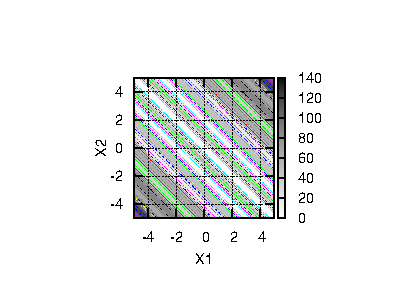
\includegraphics{multimod.eps}}
\end{minipage}
\begin{minipage}[b]{1\linewidth}
 \centering
 \resizebox*{11cm}{!}{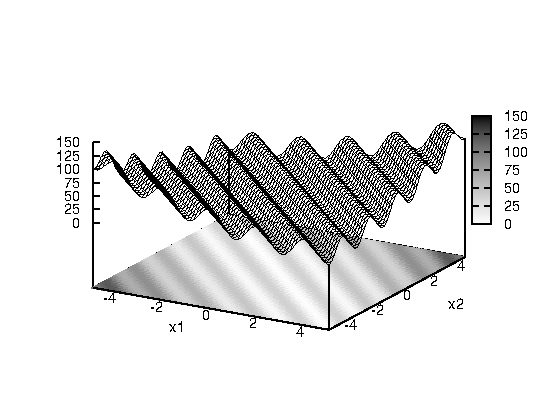
\includegraphics{multimodnomap.eps}}
\end{minipage}
\caption{Two dimensional example of the optimizations problem eq. \ref{mm}. In this example optimum value of $x_1$ is depended of the choice of $x_2$ and vice versa thus this objective function suffers from variable correlations (non-separable). If, nevertheless, one of the two design variables was aligned to the $x_1+x_2$ axis, or the $\sum^{n}_{i=1}x_i$ one in the $n$ dimensional case, the problem becomes separable.} 

\label{multimod}
\end{figure}

Observing figure \ref{multimodres} one can observe that both for the 5D and 30D problems, the separable case outperforms the non-separable one. Furthermore one can observe that the increased dimension caused an increase in the efficiency gab, between separable and non-separable cases, as shown also for the ellispoid test case. 



\begin{figure}[h!]
\begin{minipage}[b]{0.5\linewidth}
 \centering
 \resizebox*{7cm}{!}{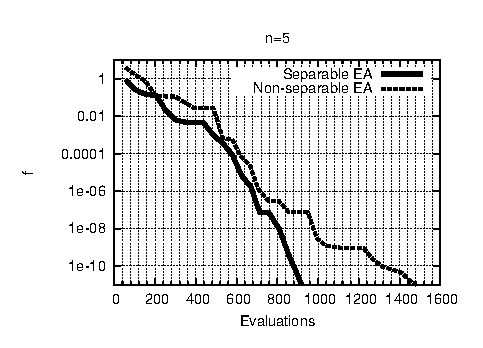
\includegraphics{5d.eps}}
\end{minipage}
\begin{minipage}[b]{0.5\linewidth}
 \centering
 \resizebox*{7cm}{!}{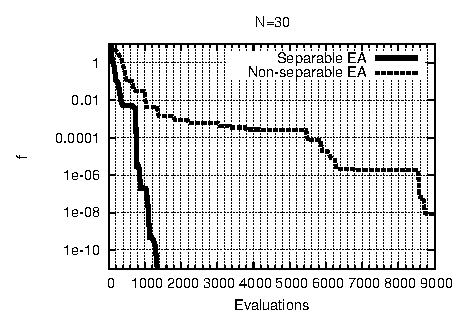
\includegraphics{30d.eps}}
\end{minipage}
\caption{Left: 5 dimensional optimization problem eq.\ref{mm}. Right: 30 dimensional optimization problem eq.\ref{mm}. The amount of efficiency losses in problems with extremely ill-conditioned objective functions increases significantly with the dimension of the design space.} 
\label{multimodres}
\end{figure}

Through the investigations of the effects of variable correlation presented in figs. \ref{ellipse_t1}, \ref{ellipse_t2} and \ref{multimodres} it is proven that a significant amount of EA effitiency can be lost when they are dealing with optimization problems with correlated design variables. The severity of efficiency deterioration is analogous to three main quantities;

\begin{description}
  \item[a)] The condition number, which is a measure of the non-homogeneous contribution of each design variable on the objective function thus a measure of the condition state of the problem in hand \ref{IllCon}. The bigger the condition number gets the bigger loss of EA efficiency is observed (fig. \ref{ellipse_t1} and \ref{ellipse_t2}).    
  \item[b)] Separability. Optimization problems with separable design variables can be solved significantly faster, using an EAs, as it is shown in figs. \ref{ellipse_t1}, \ref{ellipse_t2} and \ref{multimodres}.  
  \item[c)] The number of design variables $n$. Though it is obvious that increasing the number of design variables will also increase the design space thus require more resources for any stochastic search algorithm to locate the optimum solution, what is of interest in this section is that by increasing $n$ the losses generated from non-separability are magnified as well(fig. \ref{multimodres}).  
\end{description}
\section{Variable correlations in MOO}
\label{VCMM}
Regarding design variable correlations in MOO problems one should observe the shape of the scalar cost faction $\Phi$, since this is the value that drives the evolution operators, and not each and every objective function separably. In MOO variable correlations are typically in the form of non-separable extremely ill-conditioned state. This results from the fact that a Pareto front of optimal non-dominated solutions is sought. If the $\Phi$ assignment technique is based on Pareto dominance all members of the current front of non-dominated solutions have $\Phi=0$ (or very small values compared to the dominated members of the population) thus;
\begin{eqnarray}
   \mbox{Pareto front} \Rightarrow 	\Phi(\vec{f})=0  
   \label{Corr-Par} 
\end{eqnarray}
because $\vec{f}=\vec{f}(\vec{x})$,
\begin{eqnarray}
	\Phi(\vec{f}(\vec{x}))=0 \Rightarrow \Phi^*(\vec{x})=0
    \label{Corr-Par2}
\end{eqnarray}
where $\Phi^*$ is the direction in design space with the bigger variance.

An analytical form of $\Phi^*$ is, in the general case, very difficult to calculate due mainly to the non analytical form of $\Phi$ (eq.\ref{SPEAIIeq}) and the complex mapping form objective space to design variable space. In this thesis a method that can estimate, with increasing accuracy as the evolution proceeds, the variable correlations without calculating the analytical form of $\Phi^*$ is proposed. Further more new evolution operators are proposed to utilize this information in an EA frame.  

%\begin{figure}[h!]
%\begin{minipage}[b]{1\linewidth}
% \centering
% \resizebox*{10cm}{!}{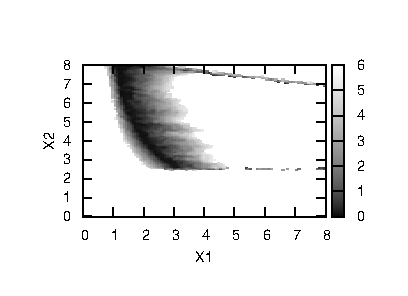
\includegraphics{CaseCorr.eps}}
%\end{minipage}
%\caption{Example $\Phi'$ plot for} 
%\label{phi1}
%\end{figure}
\section{Variable correlation estimation}
Since the current front of non-dominated solutions "elite-set" ($\Phi=0$) is the best so far approximation of the actual Pareto front it can be used to estimate the variable correlations. This estimations are as close to the real correlations as close as the current elite-set is to the actual Pareto front. Therefore dynamically updated variable correlations estimation as the elite-set increases in quality is proposed. To extract the internal structure of the elite-set in the design variable space without computing an analytical formula and in a way which best explains the variance principal component analysis (PCA) is used. 
 
PCA is an eigenvector--based multivariate analysis, performed on a data--set, that transforms possibly correlated variable sets into uncorrelated ones known as principal components. The latter are the direction vectors that best represent the variance in the data--set, \cite{Haykin,Jolliffe_2002}.
 
By assuming the current elite set to be a standardized data--set ($X$) with the empirical covariance matrix, \cite{Fodor_2002, Jolliffe_2002},

\begin{equation} 
   P_{N\times N}= \frac{1}{e}XX^T
   \label{Cov_Mat} 
\end{equation}
where $e$ is the size of $S_e$, we can use the spectral decomposition theorem, \cite{Axler_1997, Fodor_2002}, to write $P$ as

\begin{equation} 
   P_{N\times N}= U\Lambda U^T
   \label{spectral}
\end{equation}
where $\Lambda\!=\!diag(\lambda_1 , . . . , \lambda_n )$ is the diagonal matrix with the eigenvalues of $P$ and $U$ is a $N\!\times\!N$ matrix containing the eigenvectors also known as principal components or directions. 

In this PhD thesis it is proposed that the principal directions, as they are computed via PCA on the elite-set in order to best represent the variance in it, are also the directions in the search space that have the biggest degree of separability between them as far as the optimization problem in hand is concerned 

To better demonstrate the variable correlation estimation in MOO problems  the welded beam test case is used (fig. \ref{case}).  The minimization of both the cost ($K$) and the deflection ($\Delta$) of a welded beam subject to a force $P$ (fig. \ref{case}) is desired. There are two design variables: the welding length ($X_1$)  and the side length of the square cross section ($X_2$) (fig. \ref{case}). The design is subject to constraints of shear stress ($\tau$), bending stress ($\sigma$) and buckling load ($P_c$).    

\begin{figure}
\begin{minipage}[b]{1\linewidth}
 \centering
 \resizebox*{5cm}{!}{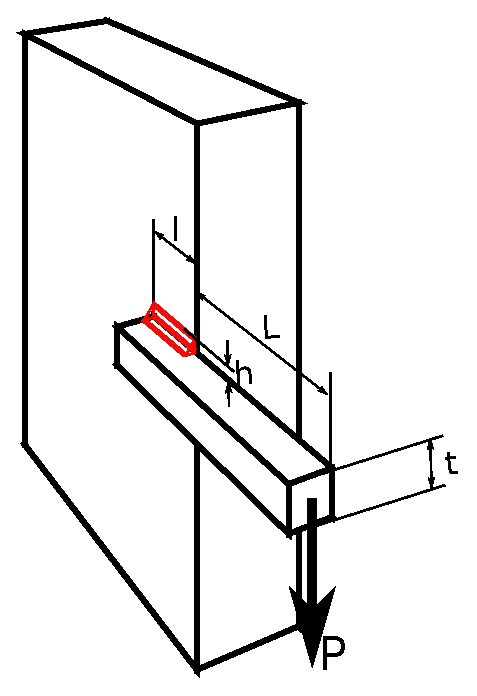
\includegraphics{case.eps}}
\end{minipage}
\caption{In the examined case, design variables are square cross section side-length ($X_2 = t$) and welding length ($X_1 = l$) are the design variables.} 
\label{case}
\end{figure}

%\figuremacroW{case}{Welded beam case - Problem definition.}{In the examined case, design variables are square cross section side-length ($X_2 = t$) and welding length ($X_1 = l$) are the design variables.}{0.4}

The problem is formulated formulated as,

Minimize Cost,
%\begin{equation} 
\begin{eqnarray}\nonumber
   K = 1.10471h^2l+0.04811t^2(14.0+l) \\
   = 1.10471h^2X_1+0.04811X_2^2(14.0+X_1)
   \label{Cost} 
\end{eqnarray}
and minimize Deflection,
%\end{equation}
\begin{eqnarray}
   \Delta = \frac{4PL^3}{Et^4} = \frac{4PL^3}{EX_2^4}
   \label{Deflection} 
\end{eqnarray}

Subject to:


Constraint concerning the shear stress applied on the welding in order to ensure the structural integrity of the welding. Maximum shear stress depends on the type and quality of the welding. 
\begin{eqnarray}
   \tau = \sqrt{\tau_1^2 + \frac{\tau_1 \tau_2 l}{R} +\tau_2^2} \\
   \nonumber \tau \leq 13,600 psi \\
   \nonumber where:~~~~~~~~~~~~~~~~~~~~~~.\\
   \nonumber \tau_1 = \frac{P}{\sqrt{2}hl} \\
   \nonumber \tau_2 = \frac{MR}{J} \\   
   \nonumber M = P(L+\frac{l}{2}) \\ 
   \nonumber R = \sqrt{\frac{l^2}{4} + (\frac{h+t}{2})^2} \\
   \nonumber J = 2\left( \sqrt{2}hl\left( \frac{l^2}{12} + \left(\frac{h+t}{2}\right)^2 \right) \right)
   \label{shear} 
\end{eqnarray}

concerning the bending stress applied on the beam, to ensure structural integrity of the beam. Maximum bending stress depends on the beam material.
\begin{eqnarray}
   \sigma = \frac{6PL}{t^3} \leq 30,000 psi
   \label{bend} 
\end{eqnarray}

and concerning the buckling load, to avoid buckling phenomena.  
\begin{eqnarray}
   P_c = \frac{4.013E\sqrt{\frac{t^8}{36}}}{L^2}\left( 1- \frac{t}{2L}\sqrt{\frac{E}{4G}} \right) \\
   \nonumber  P - P_c \leq 0 
   \label{back} 
\end{eqnarray}
where welding hight is $h = 0.6 in$, beam reach is $L = 14 in$, the extend of the force is $P = 6000 lb$, Young’s modulus is $E = 30 \times 10^6 psi$, and shear modulus is $G = 12 \times 10^6 psi$.  

Apart from the structural, constraints are also enforced on the objectives to bound the Pareto front within logical values, thus:

\begin{eqnarray}
   K \leq 50 \\
   \Delta \leq 0.25 
   \label{obj} 
\end{eqnarray}


\begin{figure}[h!]
%\begin{minipage}[b]{0.5\linewidth}
% \centering
% \resizebox*{7cm}{!}{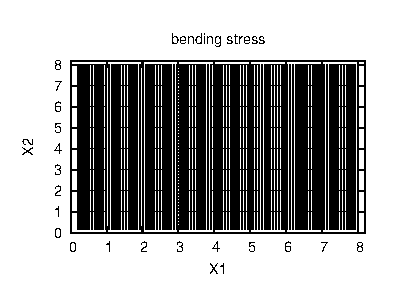
\includegraphics{Const_sx.eps}}
%\end{minipage}
%\begin{minipage}[b]{0.5\linewidth}
% \centering
% \resizebox*{7.5cm}{!}{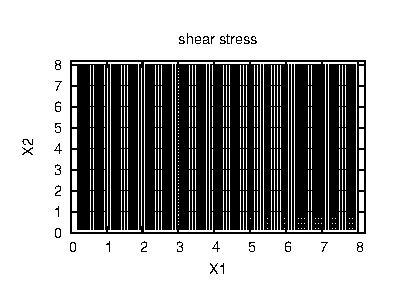
\includegraphics{Const_tx.eps}}
%\end{minipage}
%\begin{minipage}[b]{0.5\linewidth}
% \centering
% \resizebox*{7.5cm}{!}{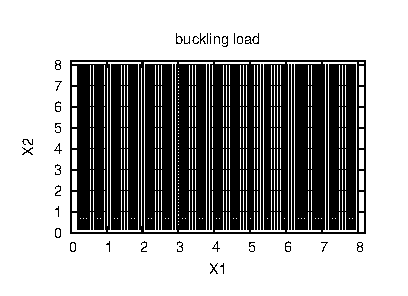
\includegraphics{Const_P.eps}}
%\end{minipage}
%\begin{minipage}[b]{0.5\linewidth}
% \centering
% \resizebox*{7.5cm}{!}{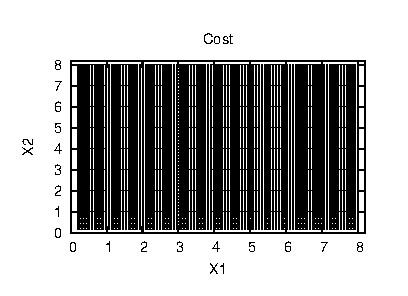
\includegraphics{Const_Price.eps}}
%\end{minipage}
%\begin{minipage}[b]{0.5\linewidth}
% \centering
% \resizebox*{7.5cm}{!}{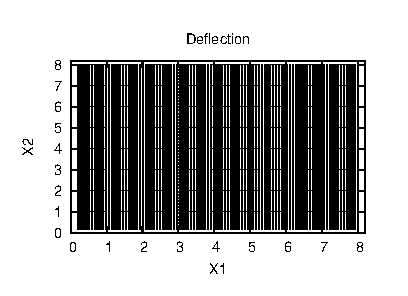
\includegraphics{Const_Dx.eps}}
%\end{minipage}
\begin{minipage}[b]{1\linewidth}
 \centering
 \resizebox*{12cm}{!}{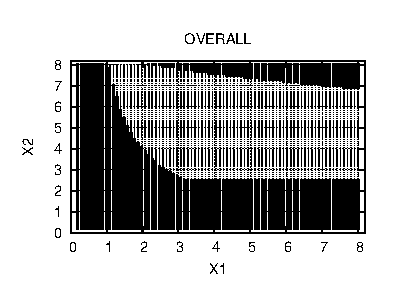
\includegraphics{Const_ALL.eps}}
\end{minipage}

\caption{Investigation of the feasibility of the design $(X_1,X_2)$ plane. The overall feasible design space is presented in the lower right figure with white squares.} 
\label{x1x2}
\end{figure}

%This case was deliberately chosen as a demonstration case due to the clear physical meaning of the relations that appear between its design variables. By carefully examining the objectives it is clear that in order to decrease deflection $X_1$ must be increased(eq. \ref{Deflection}). However any increase in $X_1$ will lead to higher cost (eq. \ref{Cost} ). In order to keep cost stable $X_2$ must simultaneously decrease, this of-course is bounded by the structural constraints (eq. \ref{shear},\ref{bend} and \ref{back}). 
 
Observing the shape of $\Phi$ in figure \ref{reco1}-left it is evident that the problem in hand is, both, extremely ill-conditioned and non-separable as expected. Using, the proposed in this PhD thesis, variable correlation estimation procedure via applying PCA on the elite-set (fig. \ref{reco1} -right) it is obvious that the principal directions, as they are computed from PCA, are pointing out the separable directions in the design space. The direction with the biggest eigenvalue $e_1$ is the direction that describes the Pareto front, walks along $\Phi=0$. On the other hand the principal direction with the smallest eigenvalue $e_2$ is the direction in the design space that yields the biggest change in $\Phi$ values. Smaller eigenvalue means smaller variance in this direction thus the EA, through its evolution operators, restricted the values of this direction within a small band of values denoting the importance regarding $\Phi$ for the this direction. 

Looking at the physical meaning of the correlations between the design variables in the welded beam case; $e_1$ suggest that if one desires to move along the  $\Phi=0$ front he should either increase $X1$ (welding length) and decrease $X2$ (cross section) or vise vesra. In other words one can move from, say, expensive designs with small deflection to cheap designs with bigger deflection (fig.\ref{Pareto1}) by reducing the cross section but in order to keep respecting the various stress constraints (fig.\ref{x1x2}) one should simultaneously increase the welding length. On the other hand $e_2$ suggest that if one wants to move on the direction that would cause the biggest difference in $\Phi$ he should either increase both $X1$ \& $X2$ or decrease them together.          

\begin{figure}[h!]
\begin{minipage}[b]{1\linewidth}
 \centering
 \resizebox*{!}{4.5 cm}{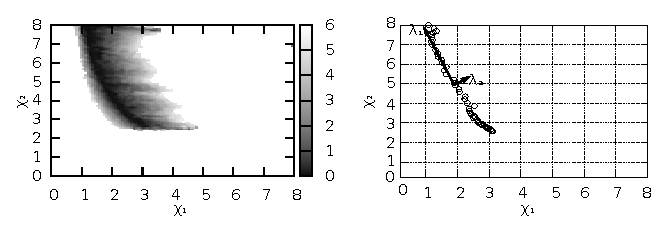
\includegraphics{DOFs.eps}}
\end{minipage}
%\begin{minipage}[b]{0.5\linewidth}
% \centering
%\resizebox*{8cm}{!}{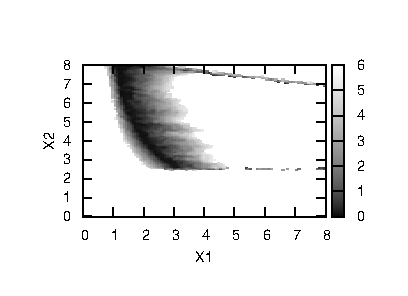
\includegraphics{CaseCorr.eps}}
%\end{minipage}
\caption{Left. $\Phi$ plot over the design space of the welded beam test case. $\Phi = 0$ suggest the presence of variable correlations. Right. Elite-set plotted on the design space and computed principal directions $e_1$ and $e_2$.} 
\label{reco1}
\end{figure}

\begin{figure}[h!]
\begin{minipage}[b]{1\linewidth}
 \centering
 \resizebox*{!}{6 cm}{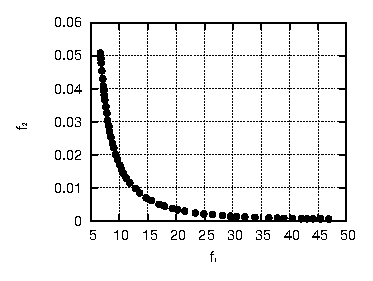
\includegraphics{Pareto.eps}}
\end{minipage}
\caption{Elite-set of fig.\ref{reco1} plotted on the objective space. F1 = cost and F2 = deflection.} 
\label{Pareto1}
\end{figure}


\section{PCA driven evolution operators} 
The PCA driven evolution operators to better ``drive'' evolution by utilising the information about the design variable correlations are proposed here as a method to deal with non-separable \& ill-conditioned optimization problems. To be more specific, PCA is used to identify the relations in the form of direction in the design space. The design space is, then, temporarily aligned with these directions, the necessary evolution operators apply to the so--rotated space and, finally, the generated offspring are transformed back to the original design space. Any sort of dimensionality reduction or rotation of the design space occurs just before (and after) the application of the evolution operators. To initiate PCA, a small number of representative solutions to the problem must be available; this set is dynamically updated during the evolution. In MOO applications, this comprises the members of the current front of non--dominated solutions. In SOO problems, in which there is no set of non--dominated solutions, the principal components can be found by processing a user--defined number of top individuals in the current offspring population. It is evident that, as the evolution proceeds, and the current front of non--dominated solutions converges to the Pareto front, the principal components approach those of the Pareto front. 

Let the aligned to the principal components design vectors \(\vec{x}_i\) be represented by \(\vec{x}^*_i\). The alignment is performed as follows
\begin{equation} 
   \vec{x}^*_i=U(\vec{x}_i-\mu_{X})
   \label{align} %http://users.ics.tkk.fi/jhollmen/dippa/node30.html
\end{equation}
where $\mu_{X}$ is the vector of mean (over the elite set) design variables.
The inverse transformation, from $\vec{x}^*_i$ to $\vec{x}_i$, is given by
\begin{equation} 
   \vec{x}_i=U^{-1}\vec{x}^*_i+\mu_{X}
	\label{re-align}
\end{equation}
It is important to note that the CPU cost to compute \(U^{-1}\) is negligible since U is an orthogonal matrix and, thus, \(U^{-1} = U^T\). 

The two main PCA driven evolution operators, recombination and mutation, are presented below.  

\paragraph{}
\subsection{PCA driven recombination}
In PCA driven recombination, the recombination operator is applied on a continuously updated design space which is sought to be as separable as possible. This, as can be seen in fig.\ref{reco2}, changes the probability of the offspring appearance on the design space in a way that  
yields higher probability to individuals that respect the aforementioned correlations between the design variables (fig.\ref{reco1}). 

\begin{figure}[h!]
\begin{minipage}[b]{0.5\linewidth}
 \centering
 \resizebox*{7cm}{!}{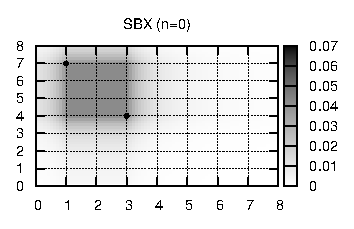
\includegraphics{SBX3dparents2a.eps}}
\end{minipage}
\begin{minipage}[b]{0.5\linewidth}
 \centering
 \resizebox*{7cm}{!}{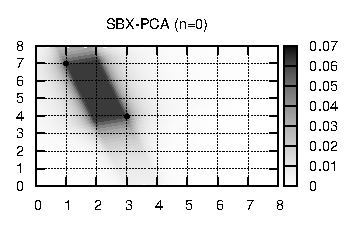
\includegraphics{SBX3dparentsPCAa.eps}}
\end{minipage}
\caption{Offspring appearance probability of the welded beam case, parents are the tow black dots. Left: SBX recombination (section \ref{RecombinationLabel}). Right: PCA driven SBX recombination. The variable correlations for the welded beam case are shown in fig.\ref{reco1}.} 
\label{reco2}
\end{figure}

Observing fig.\ref{reco1} together with fig.\ref{reco2}, it is evident that the proposed method assigns higher probability to the regions near $\Phi=0$ which is the region that accommodates the currently best (elite) individuals. Therefore recombination better achieves its goal of mixing according to the building block hypothesis \cite{Gold89}. Mixing is the process where recombination combines building blocks (low order schemata of high fitness) to form new potentially fit schemata of higher order. The proposed method, simply, increases the probability of the resulting from recombination individuals to be fit.   

%\begin{figure}[h!]
%\begin{minipage}[b]{1\linewidth}
% \centering
% \resizebox*{10cm}{!}{\includegraphics{ellipseturn_eig.eps}}
%\end{minipage}
%\caption{Example $\Phi'$ plot for} 
%\label{phi1}
%\end{figure}


\subsection{PCA driven mutation}
Mutation is also applied on the aligned with principal directions design space. Furthermore the mutation probability on each principal direction is dynamically updated based on the variance ($\vec{V}$) among the members of the elite population on the aforementioned direction ($V(i)$) eq.\ref{alignMut}. This is done in such a way that overall mutation probability per individual is kept constant (and equal to a user defined value) but the way the mutation probability is distributed among the design variable (or, to be more precise, the direction in the design space) is analogous to their importance regarding $\Phi$. As shown through the welded beam case, the importance of each principal direction regarding $\Phi$ is inversely proportional to its eigenvalue/variance therefore the principal direction with higher eigenvalues receive a smaller portion of the overall mutation probability as opposing to the directions with lower eigenvalues that receive a bigger portion of it.        

\begin{equation} 
   P_m^{i}=0.1 P_m + \frac{0.9 P_m N}{P_m^{gl}} (1-\frac{(V(i)-min(\vec{V}))}{(max(\vec{V})-min(\vec{V}))}),~~~~i=1,N 
   \label{alignMut} %http://users.ics.tkk.fi/jhollmen/dippa/node30.html
\end{equation}
where $P_m$ is the user-defined mutation probability, N the number of design variables and 
\begin{equation} 
   P_m^{gl}=\sum^{N}_{i=1} 1-\frac{(V(i)-min(\vec{V}))}{(max(\vec{V})-min(\vec{V}))}
   \label{alignMut2} %http://users.ics.tkk.fi/jhollmen/dippa/node30.html
\end{equation}


The PCA--driven MAEA or MAEA(PCA) (fig.\ref{MAEAPCA2}) algorithm is presented below. 
Let us denote the generation counter by $g$, the number of current entries into the DB by $k_{DB}$ and the minimum number of entries needed to initiate the use of the metamodel--based pre--evaluation phase by $k_{min}$. Then, the steps of the PCA--driven MAEA can be described as follows:
\begin{description}
  \item[Step 1:] For the current offspring population $S^{g}_\lambda$, set $\lambda^*\!=\!\lambda$ (if $k_{DB}\!<\!k_{min}$) or  $\lambda^*\!=\!\lambda_{ex}$ (else). 
  \item[Step 2:] If $k_{DB}\!\ge\!k_{min}$, train $\lambda$ RBF networks on paired input--output patterns selected from the DB, in the vicinity of each offspring. Pre--evaluate the $\lambda$ population members on the so--trained metamodels. Select the $\lambda_{ex}$ top of them, based on dominality and proximity criteria.
  \item[Step 3:] Evaluate the $\lambda_{ex}$ offspring on the problem--specific evaluation software. Update $S^{g}_e$.
  \item[Step 4:] Compute the current set of principal components based on the updated elite set $S^{g}_e$ (eqs. \ref{Cov_Mat} and \ref{spectral}).
  \item[Step 5:] Align the design space to so--computed principal components (eq. \ref{align}). 
  \item[Step 6:] Create the new offspring population $S^{g+1}_\lambda$ through the application of the evolution operator on the aligned individuals. Re--align the generated offspring to the original design space coordinate system,(eq.~\ref{re-align}).
  \item[Step 7:] Set $g\!\leftarrow\!g\!+\!1$; go to step 1.
\end{description}
The above algorithm can readily be transformed to EA(PCA) by eliminating the use of metamodels or by setting $k_{min}$ to a practically infinite number.  
%\figuremacroW{MAEAPCA2}{MAEA-PCA}{Schematic representation of the PCA-driven MAEA algorithm.}{1.0}
\begin{figure}[h!]
\begin{minipage}[b]{1\linewidth}
 \centering
 \resizebox*{10cm}{!}{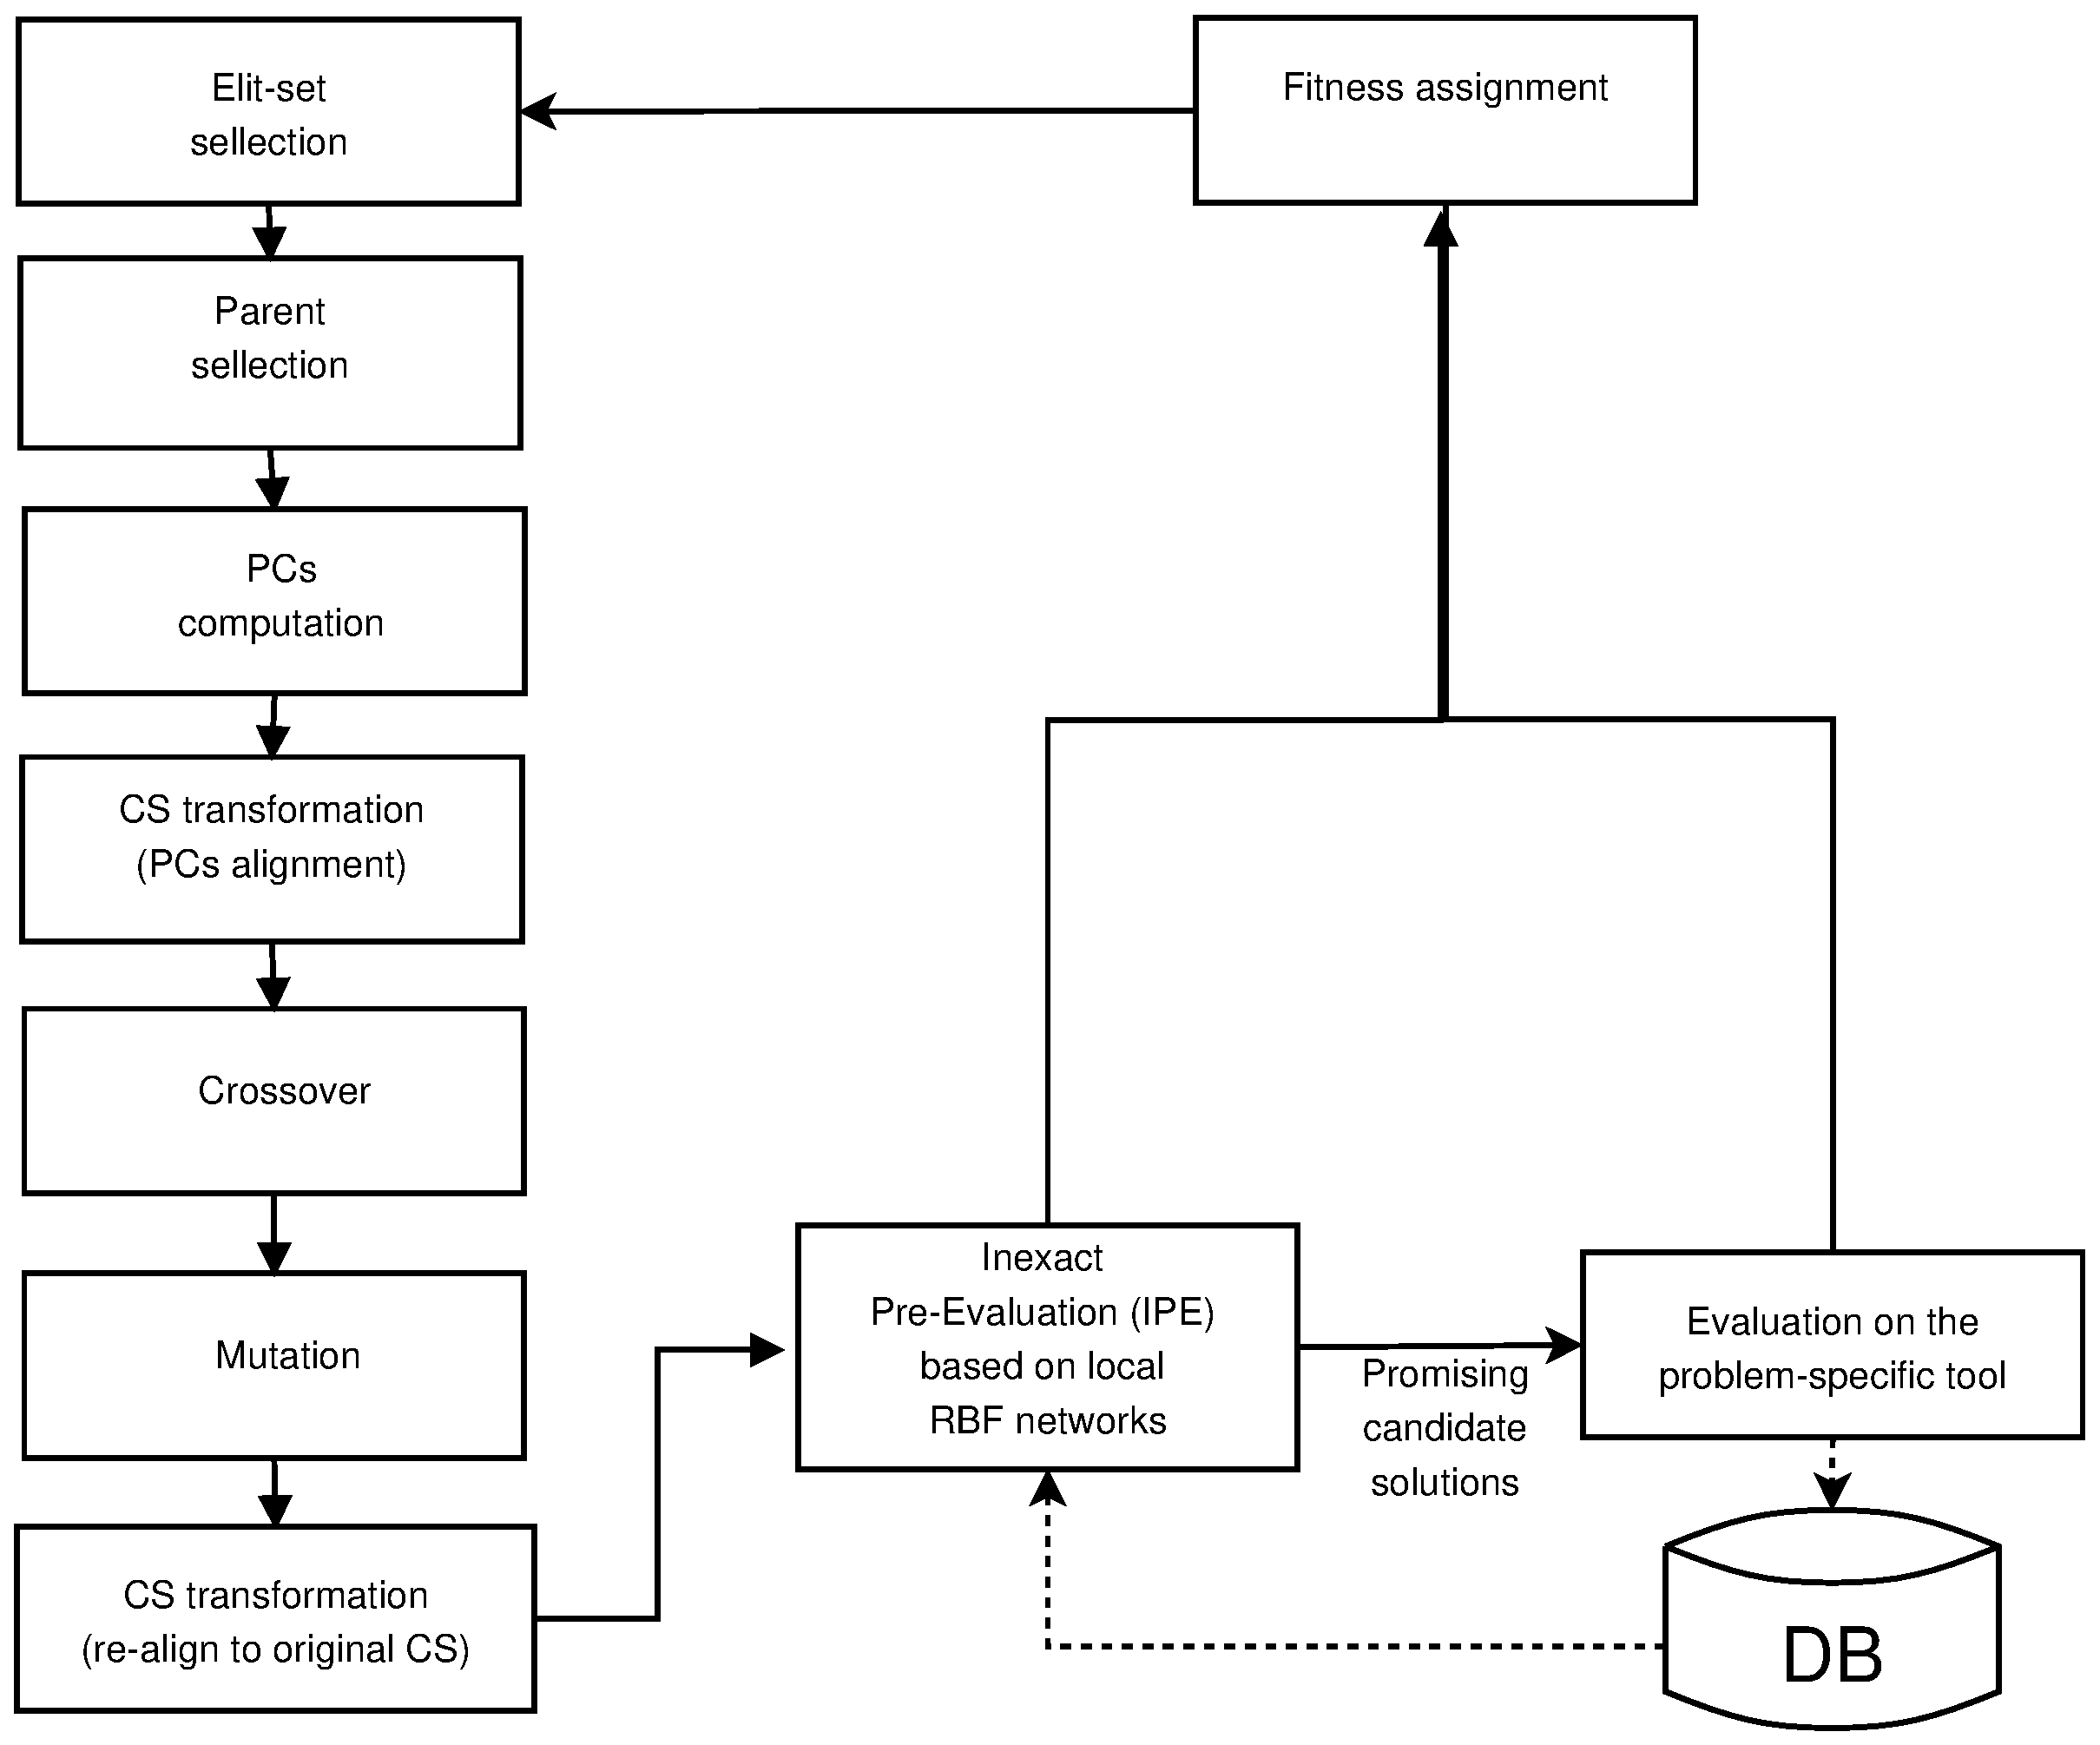
\includegraphics{MAEAPCA2.eps}}
\end{minipage}
\caption{Schematic representation of the PCA-driven MAEA algorithm.} 
\label{MAEAPCA2}
\end{figure}


%\figuremacroW{HypervolumeComparison}{Hypervolume Comparison}{Hypervolume comparison between EA and EA(PCA), metamodels where not used due to the fast evaluation time of the welded beam case. EA(PCA) outperforms traditional EA even though the dimensionality of the problem in hand is very low.}{0.9}

\subsection{Investigation of the effects of the use of PCA-driven evolution operator in ill-conditioned non-separable optimization problems}

In order to demonstrate the possible performance gain from the use of the PCA-driven EA ten runs for the aforementioned (Welded beam) case and the two mathematical test cases presented in section \ref{Inv2} were performed with different random number generator seeding. The results fo them are presented below. 

Regarding the welded beam test case the average hypervolume indicator in respect to evaluations, over the ten runs, is presented in fig. \ref{HypervolumeComparison}. 

\begin{figure}[h!]
\begin{minipage}[b]{1\linewidth}
 \centering
 \resizebox*{10cm}{!}{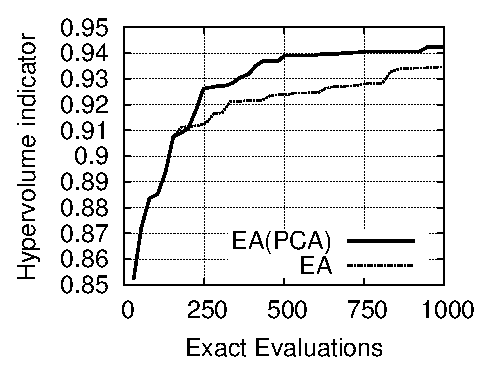
\includegraphics{HypervolumeComparison.eps}}
\end{minipage}
\caption{Hypervolume comparison between EA and EA(PCA), metamodels where not used due to the fast evaluation time of the welded beam case. EA(PCA) outperforms traditional EA even though the dimensionality of the problem in hand is very low.} 
\label{HypervolumeComparison}
\end{figure}

In figure \ref{HypervolumeComparison} one can observe that, even though, the dimension of the problem was deliberately set very low ($n=2$), for observability reasons, something that as shown in section \ref{Inv2} decreases the expected gain from the use of the proposed method it still outperforms the traditional EA.  

The comparison between traditional evolution operators and PCA-driven one of the 30D non-separable ellpsoid with $a=1000$ (eq. \ref{ellipse})is presented in fig. \ref{Ellt3}. The plots refer to the mean objective function values of the aforementioned $10$ runs. 

\begin{figure}[h!]
\begin{minipage}[b]{1\linewidth}
 \centering
 \resizebox*{10cm}{!}{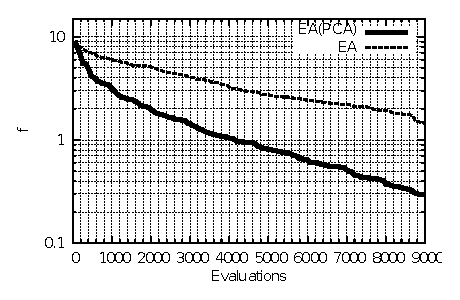
\includegraphics{1000_30d_pca.eps}}
\end{minipage}
\caption{Convergence comparison between for the 30D ellipsoid case (eq. \ref{ellipse}) with condition number ($a = 1000$). The proposed PCA-driven evolution operators significantly outperform the traditional ones.} 
\label{Ellt3}
\end{figure}

In figure \ref{Ellt3} one can observe the significant gain from the use of the proposed method in comparison with a traditional EA in the 30D ellipsoid case.

Regarding the multidimensional and multi-modal test case of eq.\ref{mm}, comparison between PCA-driven and traditional evolution operators are presented in the 30D version in fig.\ref{mmt3}.  

\begin{figure}[h!]
\begin{minipage}[b]{1\linewidth}
 \centering
 \resizebox*{10cm}{!}{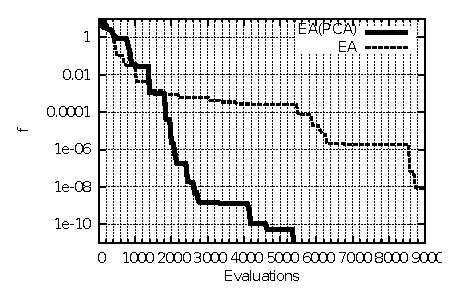
\includegraphics{30d_pca.eps}}
\end{minipage}
\caption{Convergence comparison between for the 30D multi-modal case (eq. \ref{mm}). The proposed PCA-driven evolution operators significantly outperform the traditional ones.} 
\label{mmt3}
\end{figure}

In figure \ref{mmt3} one can observe that the use of PCA-driven evolution operators significantly enhances the EA efficiency.


\section{PCA assisted metamodels}
Inexact Pre Evaluation (IPE), when using artificial neural networks (ANN) as metamodels, suffers from the curse of dimensionality. With increased dimension both the prediction accuracy decreases and the ANN training time increases. Here a method is proposed in order to reduce the $\vec{x}$ dimension in a favourable for the optimization way. As mentioned above the variable correlations are extracted via PCA performed on the members of the elite population in the form of eigenvectors, directions in the design space, and eigenvalues, variance of the corresponding direction. If a direction has big variance it means that the members of the elite population are scattered over a big range on it, that implies that this direction is of low importance for the optimization procedure. On the other hand if a direction has small variance that means that the members of the elite population are concentrated in a small region thus the direction is of big importance for the optimization.        

Since the Variable-correlations have been detected through PCA performed on the members of the elite population they could also be used to assist the metamodel training via reducing the $\vec{x}$ dimension. As mentioned  earlier in this chapter, apart from the fact that the resulting from PCA eigenvectors are the most separable directions in the design space, the eigenvalues hold information about each and every one of this directions significance to the objective function. Therefore, a truncation of $\vec{x}$ keeping only the most significant directions, is proposed in this thesis.     

To do this, first all the selected training patterns have to be rotated/aligned with the eigenvectors and then the less important (higher eigenvalues) components of them are truncated.    

In order to visually present the proposed technique the 2D welded bean case, presented earlier in this chapter, is choose. Since this is a 2D case the use of the traditional IPE technique would require the use of a 2D neural network as metamodel trained on the neighbouring to the candidate solution stored individuals as shown in figure \ref{2dann}. 
    
\begin{figure}[h!]
\begin{minipage}[b]{1\linewidth}
 \centering
 \resizebox*{15cm}{!}{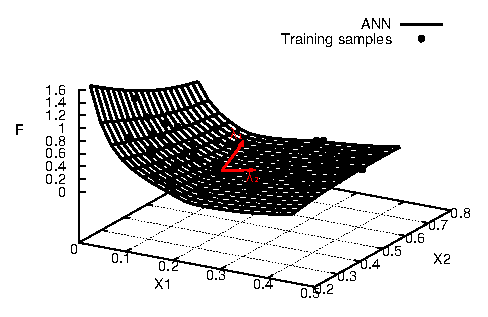
\includegraphics{2dANN.eps}}
\end{minipage}
\caption{2D ANN used as metamodel for the welded beam case and its training patterns.} 
\label{2dann}
\end{figure}

The proposed in this thesis method suggest to train only a 1D (reduced) ANN trained on the most significant regarding $\Phi$ direction (fig.\ref{1dann}-right). This is the direction with the smaller eigenvalue as it results from the use of PCA on the current elite-set. In figures \ref{reco1} and \ref{2dann} the principal directions (eigenvectors) are shown, $e_1$ denoted the principal direction with the bigger eigenvalue and $e_2$ the one with the smaller eigenvalue respectively.   

\begin{figure}[h!]
\begin{minipage}[b]{0.5\linewidth}
 \centering
 \resizebox*{7.0cm}{!}{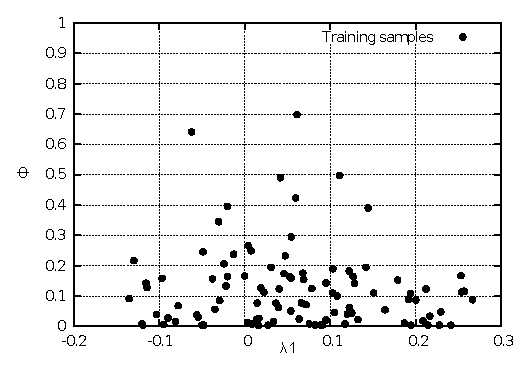
\includegraphics{1dANN_e1.eps}}
\end{minipage}
\begin{minipage}[b]{0.5\linewidth}
 \centering
 \resizebox*{7.0cm}{!}{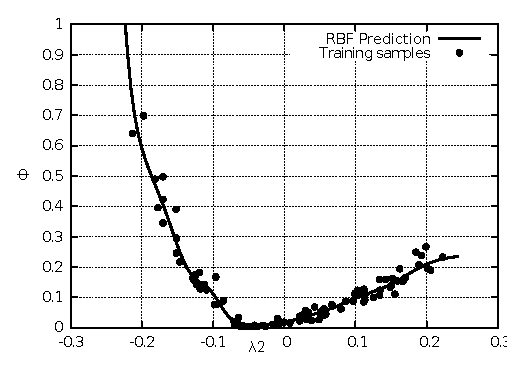
\includegraphics{1dANN_e2.eps}}
\end{minipage}
\caption{Left: the training patters projected on the ($\Phi,e_1$) plane. Right: the training patterns projected on the ($\Phi,e_2$) plane. The ANN used as metamodel by the IPE technique is trained on the ($\Phi,e_2$) plane.} 
\label{1dann}
\end{figure}

Observing figure \ref{1dann} one can see that the nature of the $\Phi$ distribution over the design space (in the vicinity the candidate solution) can be captured by the $e_2$ direction on the other hand $e_1$ direction in not that important. In fact in this case (MOO) direction $e_1$ moves along the current Pareto front approximation thus accommodates more or less designs of similar $\Phi$. The aforementioned technique is expected to add to the MAEA efficiency in cases of extremely high dimension in reducing the required DB entries before the IPE phase starts, reducing the metamodels training time and deliver favourable for the optimization predictions.     

%stelios 
\subsection{Investigation of the effects of the use of PCA assisted metamodels in ill-conditioned non-separable optimization problems}

To demonstrate the possible performance gain from the use of the proposed PCA assisted metamodels ten runs for the two mathematical test cases presented in section \ref{Inv2} were performed with different random number generator seeding. The results of them are presented below. 

Regarding comparison between traditional metamodels using PCA only to drive the evolution operators (MAEA(PCA)) and PCA assisted metamodels  or M(PCA)AEA(PCA) of the 30D non-separable ellpsoid with $a=1000$ (eq. \ref{ellipse}) is presented in fig. \ref{Ellt3-m}. The plots refer to the mean objective function values of the aforementioned $10$ runs. IPE phase for MAEA(PCA) initiated after $300$ individuals where stored in the date base and $25$ to $29$ training patterns, in the $\Re^{30}$ space, where used to train the RBF networked employed as metamodel. Regarding the M(PCA)AEA(PCA), IPE phase started after only $100$ individuals where stored in the database since only $4$ to $8$ training patterns, in the truncated  $\Re^{10}$  space, where required for the RBF network training. The $\Re^{10}$ is comprised by the $10$ most important directions in the design space according to method proposed above. 

\begin{figure}[h!]
\begin{minipage}[b]{1\linewidth}
 \centering
 \resizebox*{10cm}{!}{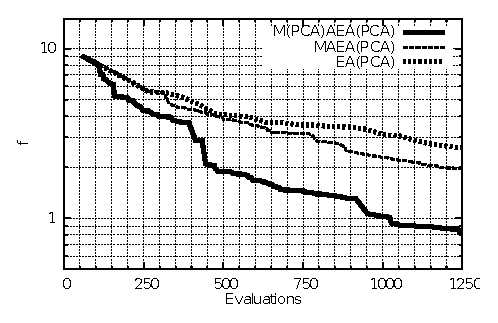
\includegraphics{1000_30d_pca_ipe.eps}}
\end{minipage}
\caption{Convergence comparison between for the 30D ellipsoid case (eq. \ref{ellipse}) with condition number ($a = 1000$). The proposed M(PCA)AEA(PCA) method outperform the MAEA(PCA) one.} 
\label{Ellt3-m}
\end{figure}


Regarding the multidimensional and multi-modal test case of eq.\ref{mm}, comparison between MAEA(PCA) and M(PCA)AEA(PCA) are presented for the 30D version in fig.\ref{mmt3m}. Regarding MAEA(PCA)  IPE phase initiated after $300$ individuals where stored in the date base and $15$ to $19$ training patterns, in the $\Re^{30}$ space, where used to train the  metamodel. As far at the M(PCA)AEA(PCA) is concerned, the training pattern dimension was truncated from $30$ to the $10$ most important regarding $f$. That allowed for the  IPE phase to start after only $100$ individuals where stored in the database since only $5$ to $9$ training patterns where required for the RBF network training.

\begin{figure}[h!]
\begin{minipage}[b]{1\linewidth}
 \centering
 \resizebox*{11cm}{!}{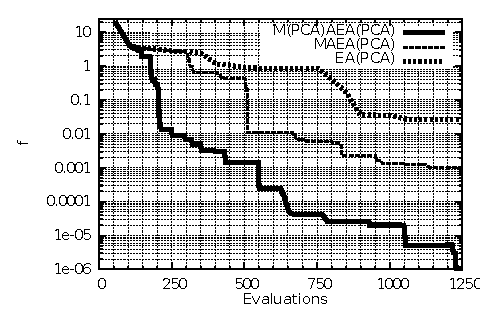
\includegraphics{30d_pca_ipe.eps}}
\end{minipage}
\caption{Convergence comparison between for the 30D multi-modal case (eq. \ref{mm}).The proposed M(PCA)AEA(PCA) method outperform the MAEA(PCA) one.} 
\label{mmt3m}
\end{figure}

In figure \ref{mmt3} one can observe that the use of PCA assisted metamodels significantly enhances the IPE phase efficiency.

%stelios

\section{Design of a compressor cascade using the proposed M(PCA)AEA(PCA) method}


The design of a two dimensional compressor cascade operating at $M_1=0.54$, $a_1=44^o$ and $Re=4\times10^5$ for minimum total pressure losses ($\omega$) eq.\ref{omegaLosses} is sought. 

The blade airfoil is designed subject to a number of aerodynamic and geometrical constraints: the optimal airfoil must turn the flow by more than $30^o$ and ensure that its thickness at three chord-wise positions ($0.3c$, $0.6c$ \& $0.9c$) must be greater that ($0.10c$, $0.08c$ \& $0.01c$)  respectively.     

The airfoil shape is parameterized based on a mean-camber line and thickness distributions scheme as presented in section \ref{Drela1}, a parameterization that yields $27$ design variables.

The merits of the proposed M(PCA)AEA(PCA) method will be examined through the comparison of a traditional MAEA against a M(PCA)AEA(PCA) where PCA is used both to drive the evolution operators and also during the IPE phase to reduce the metamodel dimension. The populations for both MAEAs are $\mu=20$, $\lambda=60$ and $\lambda_e=6$. Both cases use local RBF networks as metamodels trained on a small number of automatically selected training patterns. The MAEA uses a number of  $20$ to $30$ training patterns in the $\Re^{27}$ space. IPE phase for MAEA starts after $400$ individuals are stores in the database. Regarding M(PCA)AEA(PCA) the RBF networks used as metamodels are trained with $5$ to $8$ training patterns in the reduced as presented above $\Re^{10}$ space. The reduced dimension makes possible the use of metamodels significantly earlier, the IPE phase for M(PCA)AEA(PCA) starts after only $200$ individuals are stored in the database. 


\begin{figure}[h!]
\begin{minipage}[b]{1\linewidth}
 \centering
 \resizebox*{11cm}{!}{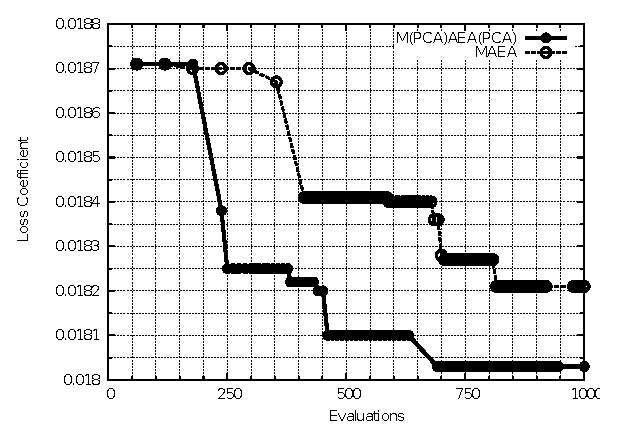
\includegraphics{CompPCA.eps}}
\end{minipage}
\caption{Convergence comparison between MAEA and M(PCA)AEA(PCA) methods.} 
\label{PCADrelaRes}
\end{figure}

Figure \ref{PCADrelaRes} shows the convergence of both methods. M(PCA)AEA(PCA) outperforms the traditional MAEA during all but the initial steps of the optimization procedure. 

\begin{figure}[h!]
\begin{minipage}[b]{1\linewidth}
 \centering
 \resizebox*{16cm}{!}{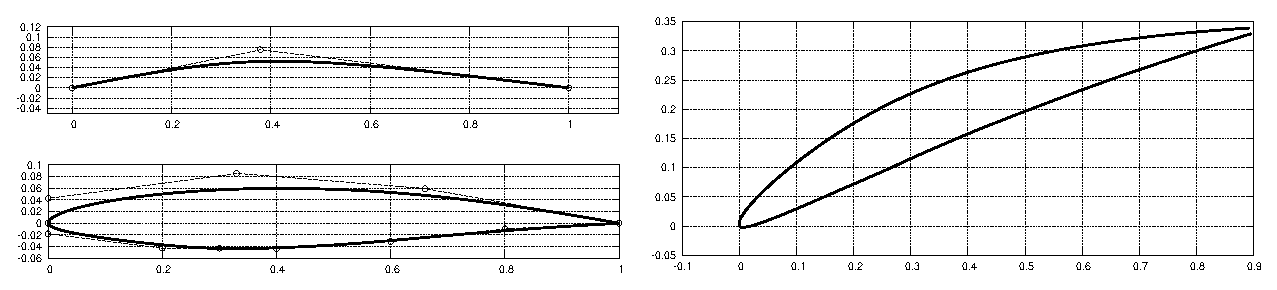
\includegraphics{ResD.eps}}
\end{minipage}
\caption{The optimal airfoil resulting form M(PCA)AEA(PCA). Left: mean camper line and thickness distribution together with their control polygons. Right: The final airfoil after superimposing thickness distribution on the mean camper line and turned accordingly with the stagger angle.} 
\label{PCADrelaRes}
\end{figure}

The optimal airfoil resulting form M(PCA)AEA(PCA) (fig. \ref{PCADrelaRes}) has total pressure losses $\omega=0.01803$ and respects both the thickness and flow turning constraints.  Flow turning of the blade in hand is $\Delta a=30^o$

\begin{figure}[h!]
\begin{minipage}[b]{1\linewidth}
 \centering
 \resizebox*{12cm}{!}{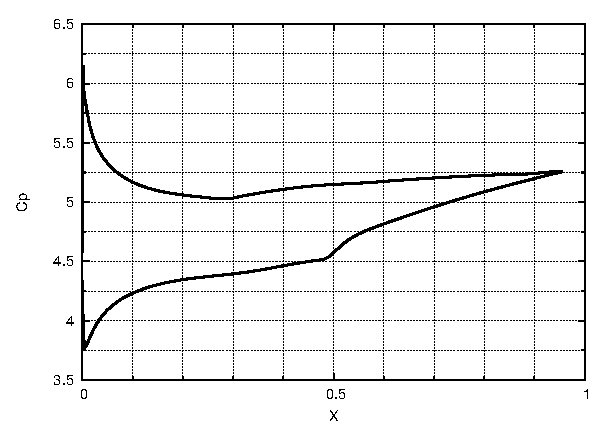
\includegraphics{Best_CP_PCA.eps}}
\end{minipage}
\caption{Pressure coefficient $C_p$ of the optimal airfoil fig.\ref{CBRDrelaRes}.} 
\label{PCADrelaRes_cp}
\end{figure}

% ---------------------------------------------------------------------------
% ----------------------- end of thesis sub-document ------------------------
% ---------------------------------------------------------------------------